\subsubsection*{Variables}
For the relativistic notation in Chapter~\ref{ch:furry_pic}, the symbols $x$, $y$, $z$, $z_1$, $z_2$, and $p$ are used for four vectors corresponding to $x^\mu=(x^0,\mathbf{x})=(x^0,x^1,x^2,x^3)$, where bold symbols stand for the three-component spacial vectors. The scalar product is $x_\mu y^\mu = x^0 y^0 - \mathbf{x}\cdot\mathbf{y}$, corresponding to the metric $g^{\mu\nu}=\text{diag}(1,-1,-1,-1)$.\\
In all other chapters, three dimensional vectors in spherical coordinates are written as bold symbols $\mathbf{r}=(r,\vartheta,\varphi)$, where $\varphi$ is the polar angle and $\vartheta$ is the azimuthal angle. The volume element is as usual $\text{d}^3\mathbf{r}=\text{d}r\text{d}\varphi\text{d}\vartheta\, r^2 \sin\vartheta $.
\subsubsection*{Feynmanrules}
In Chapter~\ref{ch:furry_pic}, the following Feynman rules in position space are needed, where the notation follows~\cite{itzykson2005}. If external lines are needed, the corresponding solutions of the Dirac equation have to be used.\\

\begin{tabular}{lll}
fermion propagator (ext. field):&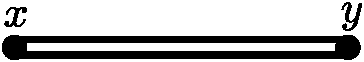
\includegraphics[width=0.2\linewidth]{pics/feynrule_1.pdf} & $S_{\mathcal{A}}(x,y)\phantom{-}$ from Eq.~\eqref{eq:extpropdef}\\[7pt]
fermion propagator (free):&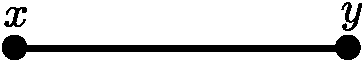
\includegraphics[width=0.2\linewidth]{pics/feynrule_2.pdf} &$S_{F}(x-y)$ from Eq.~\eqref{eq:freepropdef}\\[7pt]
photon propagator:&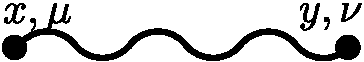
\includegraphics[width=0.2\linewidth]{pics/feynrule_3.pdf} &$g_{\mu\nu}\cfrac{1}{4\pi^2}\cfrac{1}{(x-y)^2-i\epsilon}$\\[7pt]
vertex:&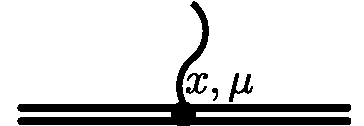
\includegraphics[width=0.2\linewidth]{pics/feynrule_4.pdf} &$-ie\gamma^\mu\int\text{d}^4x$
\end{tabular}
\subsubsection*{Dirac matrices}
The following representation of the Dirac matrices is chosen, following~\cite{greiner2000}:\\
\textit{$\beta$ and $\gamma$ matrices:}\\[-10pt]
\begin{equation}
\beta=\gamma^0 =
\begin{pmatrix}
\boldsymbol{1}&\boldsymbol{0}\\
\boldsymbol{0}&\boldsymbol{-1}
\end{pmatrix};\qquad
\gamma^{i} = 
\begin{pmatrix}
\boldsymbol{0}&\boldsymbol{\sigma}^i\\
-\boldsymbol{\sigma}^i&\boldsymbol{0}
\end{pmatrix}
\end{equation}
with\\[-10pt]
\begin{equation}
\boldsymbol{0}=
\begin{pmatrix}
0&0\\0&0
\end{pmatrix};\quad
\boldsymbol{1}=
\begin{pmatrix}
1&0\\0&1
\end{pmatrix};\quad
\boldsymbol{\sigma}^1=
\begin{pmatrix}
0&1\\1&0
\end{pmatrix};\quad
\boldsymbol{\sigma}^2=
\begin{pmatrix}
0&-i\\i&0
\end{pmatrix};\quad
\boldsymbol{\sigma}^3=
\begin{pmatrix}
1&0\\0&-1
\end{pmatrix};\quad
\end{equation}
\textit{$\alpha$ matrices:}
\begin{equation}
\boldsymbol{\alpha}^i = \gamma^0 \gamma^i =
\begin{pmatrix}
\boldsymbol{0}&\boldsymbol{\sigma}_i\\
\boldsymbol{\sigma}_i&\boldsymbol{0}
\end{pmatrix}
;\quad\text{with }i \in \{1,2,3\}.
\end{equation}
$\phantom{1}$

\subsubsection*{System of units and physical constants}
Relativistic natural units are used in this thesis, where $\hbar=c_0=1$, where $\hbar$ is the reduced Planck's constant, and $c_0$ is the speed of light in vacuum. In Chapter~\ref{ch:muonic_atoms}, relativistic muonic natural units are used, where additionally $m_\mu=1$, where $m_\mu$ is the muon mass. For example, the electron mass in this system of units has the numerical value of the mass ratio $m_e/m_\mu = 1/206.768 2826$~\cite{codata}.
Furthermore, Lorentz-Heavyside units of electromagnetism are used, corresponding to $\epsilon_0=\mu_0=1$, where $\epsilon_0$ is the vacuum permittivity and $\mu_0$ the vacuum permeability.
Table~\ref{tab:units} gives an overview of the SI-values of the basis units and derived quantities in muonic natural units.\\[1.5cm]

\begin{table}[h]
\caption{\label{tab:units}Overview of the SI-values of the basis units for the used natural systems of units and other important derived quantities. SI Values for $\hbar$, $c$, $m_\mu$, $\epsilon_0$, $\mu_0$ are taken from~\cite{codata2016}.}
\centering\setcellgapes{4pt}\makegapedcells
\begin{tabular}{lc|ll}
\\
Planck's constant &$\hbar$ & \multicolumn{2}{l}{$1.054571800 \phantom{1}\times 10^{-34} \,\text{kg m}^2 \text{s}^{-1}$} \\
speed of light &$c_0$ & \multicolumn{2}{l}{$299792458\phantom{1} \,\,\phantom{\times 1001 ^{-34}} \text{m s}^{-1}$}\\
muon mass &$m_\mu$ & \multicolumn{2}{l}{$1.883531594\phantom{1} \times 10^{-28} \,\text{kg}$}\\
vacuum permittivity &$\epsilon_0$ & \multicolumn{2}{l}{$8.854187817\phantom{1} \times 10^{-12} \,  \text{kg}^{-1} \text{m}^{-3}\text{s}^4\text{A}^2$}\\
vacuum permeability &$\mu_0$ & \multicolumn{2}{l}{$12.566370614 \times 10^{-7\phantom{1}} \,\text{kg m} \text{ s}^{-2}\text{A}^{-2}$}\\[15pt]
%electron mass &$m_e$ & \multicolumn{2}{l}{$9.10938356\phantom{0}\times 10^{-31}\, \text{kg} $}\\
%&& $m_f=m_e$ & $m_f=m_\mu$ \\\cline{3-4}
%distance & $\hbar/(mc)$ & $386.159267\times10^{-15} \,\text{m}$ & $1.86759431\times 10^{-15}\,\text{m}$\\
%time & $\hbar /(m c^2)$ & $1.28808867\times 10^{-21}\,\text{s}$ & $6.22962405\times 10^{-24}\,\text{s}$\\
%energy & $mc^2$ & $8.18710565\times 10^{-14}\,\text{J}$ & $1.69283377\times 10^{-11}\,\text{J}$\\
distance & $\hbar/(m_\mu c)$ & $1.86759431\phantom{11}\times 10^{-15}\,\text{m}$\\
time & $\hbar /(m_\mu c^2)$ & $6.22962405\phantom{11}\times 10^{-24}\,\text{s}$\\
energy & $m_\mu c^2$ & $1.69283377\phantom{11}\times 10^{-11}\,\text{kg m}^2\text{s}^{-2}$\\
\end{tabular}
\end{table}
\clearpage
